%% LyX 2.2.0 created this file.  For more info, see http://www.lyx.org/.
%% Do not edit unless you really know what you are doing.
\documentclass[11pt]{article}
\renewcommand{\ttdefault}{lmtt}
\usepackage[T1]{fontenc}
\usepackage[utf8]{inputenc}
\usepackage{geometry}
\geometry{verbose,tmargin=2.5cm,bmargin=3cm,lmargin=4cm,rmargin=2cm}
\synctex=-1
\usepackage{array}
\usepackage{float}
\usepackage{textcomp}
\usepackage{graphicx}

\makeatletter

%%%%%%%%%%%%%%%%%%%%%%%%%%%%%% LyX specific LaTeX commands.
%% Special footnote code from the package 'stblftnt.sty'
%% Author: Robin Fairbairns -- Last revised Dec 13 1996
\let\SF@@footnote\footnote
\def\footnote{\ifx\protect\@typeset@protect
    \expandafter\SF@@footnote
  \else
    \expandafter\SF@gobble@opt
  \fi
}
\expandafter\def\csname SF@gobble@opt \endcsname{\@ifnextchar[%]
  \SF@gobble@twobracket
  \@gobble
}
\edef\SF@gobble@opt{\noexpand\protect
  \expandafter\noexpand\csname SF@gobble@opt \endcsname}
\def\SF@gobble@twobracket[#1]#2{}
%% Because html converters don't know tabularnewline
\providecommand{\tabularnewline}{\\}

%%%%%%%%%%%%%%%%%%%%%%%%%%%%%% User specified LaTeX commands.
\hyphenation{MechWarrior przes-trzen-nej u-żyt-kow-ni-ka jas-ki-ni jas-ki-nia naj-waż-niej-szy-mi do-łą-czo-no u-sta-wio-ne przy-sto-so-wa-nym prze-tes-to-wa-ne}
\sloppy

\makeatother

\begin{document}
tutaj strona główna

System wizualizacji oparty o Blender w środowisku jaskini rzeczywistości
wirtualnej

\section*{\newpage{}}

tutaj pusto

\section*{\newpage{}}

tutaj spis treści

\newpage{}

\part*{Słownik}
\begin{itemize}
\item \textbf{Rzeczywistość wirtualna (ang. Virtual Reality)} - sposób użycia
technologii komputerowej do tworzenia trójwymiarowego świata, w którym
obiekty dają wrażenie przestrzennej obecności\footnote{Steve Bryson,,Virtual reality: A Definition History - A Personal
Essay'', 1998, s. 4 http://arxiv.org/pdf/1312.4322.pdf}. Do zanurzenia się w rzeczywistości wirtualnej potrzebne jest urządzenie
wyświetlające obraz.
\item \textbf{Maszyny arcade, automaty do gier} - konstrukcja służąca rozrywce,
umieszczana najczęściej w salonach gier bądź też pubach lub klubach.
Uruchomienie gry następuje w momencie wrzucenia monety bądź żetonu
w otwór wrzutowy, zabawa ograniczona jest zwykle pewnym wyznacznikiem
narzuconym przez producenta lub właściciela automatu (np. liczba prób/żyć,
przejście na wyższy poziom, zdobycie określonego celu w zadanym czasie,
ukończenie gry). Zwykle automat do gier wyposażony był w gałkę sterującą
i kilka klawiszy.
\item \textbf{CAVE (ang. Cave Automatic Virtual Environement)} - obiekt
o kształtach sześcianu służący do zanurzenia się w rzeczywistość wirtualną.
Składa się z akrylowych ekranów tylnej projekcji oraz projektorów,
rzucających obrazy na każdą ze ścian. Człowiek wewnątrz musi nosić
aktywne okulary 3D by móc oglądać dowolnie wyświetlony obiekt z każdej
strony. Wewnątrz znajdują się również kamery śledzące pozycje użytkownika
dzięki czemu obraz jest na bieżąco dostosowywany do pozycji śledzonego.
\item \textbf{Tylna projekcja (ang: Rear Screen Projection)} - projekcja
obrazu na półprzeźroczysty ekran znajdujący się między obserwatorem
a urządzeniem. Dzięki wykorzystaniu tej techniki obraz jest jaśniejszy
i bardziej wyraźny w porównaniu do klasycznej projekcji.
\item \textbf{Aktywne okulary 3D} - rodzaj okularów 3D zasilanych bateriami
by rozdzielać renderowane klatki specjalnie dla prawego i lewego oka.
Działają na zasadzie migawki: kiedy aktualnie wyświetlana klatka jest
przeznaczona dla lewego oka, prawa migawka pozostaje zamknięta i vice
versa. Przy takiej formie odbierania obrazu wyświetlacz powinien odświeżać
obraz na tyle szybko by każde z oczu otrzymywało przynajmniej 60 klatek
na sekundę (co daje łącznie odświeżanie na poziomie 120 Hz)\footnote{http://www.cnet.com/news/active-3d-vs-passive-3d-whats-better/ (dostęp:
22.05.2016)}
\item \textbf{Odświeżanie obrazu} - dla ekranów LCD jest to liczba wyświetleń
w ciągu sekundy danych dostarczonych przez procesor graficzny. Ekrany
typu CRT odświeżają obraz wytrzeliwując elektrony pobudzające luminofor
(patrz: CRT).
\item \textbf{LCD (ang. Liquid Crystal Display)} - Rodzaj ciekło-krystalicznych
wyświetlaczy gdzie obraz jest sterowany poprzez zmianę poszczególnych
pikseli lub ich grup. Panel LCD nie emituje światła sam z siebie,
dlatego wymagane jest podświetlenie by obraz stał się widoczny.
\item \textbf{CRT (ang. Cathode-Ray Tube)} - Rodzaj wyświetlaczy bazujący
na lampie obrazowej oraz dziale eletronowym. Wyświetlacz używa wiązki
elektronów wystrzeliwanej z działa do wzbudzenia świecenia luminofora.
Wiązka po wystrzeleniu przebiegała przez całą powierzchnię ekranu
wywołując świecenie i ukazując na jego powierzchni obraz.
\item \textbf{Luminofor}- związek chemiczny wykazujący luminescencję.
\item \textbf{BGE (Blender Game Engine)} - jeden z komponentów Blendera
3D. Jest to open-sourcowy silnik graficzny używany do tworzenia interaktywnych
scen w czasie rzeczywistym.
\item \textbf{HMD (Head Mounted Display)} - urządzenie wyświetlające przeznaczone
do zakładania na głowę, wyposażone w soczewki pomiędzy ekranem a okiem.
Obraz jest ustawiony tak by każde oko widziało swoją część co sprawia
wrażenie stereoskopii. Wyświetlacze HMD pozwalają zanurzyć się w rzeczywistość
wirtualną.
\item \textbf{Stereoskopia}- technika pokazywania obrazu polegająca na tworzeniu
lub uwydatnianiu jego głębii.
\item \textbf{FullHD} - standard wyświetlania obrazu wysokiej jakości. Zazwyczaj
zakłada się też, że wyświetlacz jest panoramiczny (stosunek boków
jest 16:9) i posiada rozdzielczość 1920 na 1080 pikseli. Sygnał wideo
jakości FullHD ma oznaczenie 1080p.
\item \textbf{Organiczna dioda elektroluminescencyjna, OLED (ang. Organic
Light-Emitting Diode)} - dioda wytwarzana ze związków organicznych.
Jest to również oznaczenie klasy wyświetlaczy graficznych zbudowanych
na diodach OLED. W przeciwieństwie do ekranów LCD, OLED nie wymaga
dodatkowego podświetlenia i emituje światło sam z siebie co pozwala
na uzyskanie prawdziwej czerni i lepszego kontrastu\footnote{http://www.oled-info.com/introduction (dostęp: 22.05.2016)}.
\item \textbf{Immersja} - Odczuwanie, wczuwanie się w świat cyfrowy. Proces
zanurzenia się w ukazywanej, nierealnej rzeczywistości.
\item \textbf{Protokół SSH (ang. Secure Shell)} - zaszyfrowany protokół
sieciowy pozwalający na zdalne logowanie do innych komputerów w obrębie
danej sieci. Jest następną protokołu telnet, który przesyłał niezaszyfrowane
hasła i inne informacje.
\item \textbf{Finansowanie społecznościowe (ang. Crowdfunding)} - Źródło
kapitału dostarczanego przez szeroką społeczność wirtualną, która
chce wesprzeć kreatywnego pomysłodawcę\footnote{http://crowdfunding.pl/crowdfunding-faq/ (dostęp: 22.05.2016)}.
Akcje zbiórki organizowane są zazwyczaj na platformach internetowych
gdzie pomysłodawca przedstawia swój projekt. Każdy może wesprzeć dowolną
kwotą pomysłodawcę.
\item \textbf{6DoF (ang. six degrees of freedom - 6 stopni swobody)} - możliwości
wykonania ruchu przez ciało w przestrzeni trójwymiarowej. Dla 6. stopni
swobody są to:

\begin{itemize}
\item przesunięcie góra/dół względem osi X
\item przesunięcie góra/dół względem osi Y
\item przesunięcie góra/dół względem osi Z
\item rotacja względem osi X
\item rotacja względem osi Y
\item rotacja względem osi Z
\end{itemize}
\item \textbf{Podwójne buforowanie obrazu metodą Page Flipping -}metoda
rysowania i wyświetlania klatek wykorzystująca dwa osobne bufory w
pamięci. Gdy jeden z nich wyświetla gotową klatkę drugi rysuje kolejną.
Kiedy operacje rysowania klatki są zakończone następuje przełączenie
pomiędzy wyświetlaniem buforów.
\item \textbf{Poczwórne buforowanie (ang: Quad buffering)} - stereoskopiczna
implementacja podwójnego buforowania. W tym przypadku mamy 4 bufory,
z czego po dwa przydzielone są do rysowania obrazu dla jednego oka.
Operacja podmiany aktualnie wyświetlanego bufora jest jednoczesna
dla buforów prawego i lewego oka.
\item \textbf{Video Wall}- specjalny zestaw kilku lub więcej wyświetlaczy
ułożonych jeden przy drugim. Tworzą w ten sposób jeden duży ekran.
Wyświetlacze wykorzystywane przy budowie video walla zazwyczaj mają
jak najcieńszą ramę dookoła ekranu by zminimalizować przerwy pomiędzy
ekranami\footnote{http://www.pixell.com/what\_is\_a\_vw.htm (dostęp: 22.05.2016)}.
\end{itemize}

\part*{\newpage{}Wstęp}

Niniejsza praca ma na celu rozszerzenie możliwości wykorzystania jaskini
wirtualnej rzeczywistości CAVE poprzez implementację silnika graficznego
Blender Game Engine w Laboratorium Zanurzonej Wizualizacji Przestrzennej
znajdującego się na Politechnice Gdańskiej. Wykorzystując aplikację
BlenderVR każda scena odpowiednio zaprogramowana i zaprojektowana
w BGE może zostać wyświetlona w jaskini wirtualnej rzeczywistości
lub na architekturze odpowiednio podobnej. Aplikacja BlenderVR jak
i Blender3D są programami open-source. Dzięki temu systemy typu CAVE
mogą rozwijać się bardziej dynamicznie wraz z dedykowanymi dla nich
scenami lub grami. Aktualnie głównymi silnikami graficznymi, które
wykorzystywane są w Laboratorium Zanurzonej Wizualizacji Przestrzennej
są Unity i Unreal Engine. Oba zostały przystosowane do pracy w jaskiniach
wirtualnej rzeczywistości. Nie są one jednak programami open-source
co nie pozwala na dokładne dopasowanie do potrzeb laboratorium. Wykorzystanie
nowej opcji jaką jest Blender Game Engine rozszerzy możliwości modelowania
scen dedykowanych dla CAVE’a.

\pagebreak{}

\part{Technologia wirtualnej rzeczywistości}

Wirtualna rzeczywistość od zawsze intrygowała człowieka. W wielu filmach
czy książkach wizje przyszłości często zawierały urządzenia pozwalające
oderwać się od rzeczywistości i w pełni zanurzyć się w dowolnie ukształtowanym
świecie wirtualnym. Teraźniejszość coraz bardziej zaczyna przypominać
tę przyszłość.

Pierwsze wzmianki o rzeczywistości wirtualnej mogą pochodzić z lat
30. XX wieku. Terminu,,la réalité virtuelle'' użył Antonin Artaud
w swoim zbiorze esejów pod tytułem,,Le Théâtre et son double''.
Jako rzeczywistość wirtualna została opisana iluzjonistyczna natura
postaci i obiektów w teatrze\footnote{http://www.almaclassics.com/excerpts/Theatre\_Double.pdf (dostęp 07.05.20016)}.
To co dzisiaj kryje się pod nazwą rzeczywistości wirtualnej było popularyzowane
dopiero przez media masowe w filmach takich jak:,,Brainstorm'' i,,The
Lawnmover Man''. Pierwszym urządzeniem, które można by nazwać systemem
VR była Sensorama\footnote{http://www.theverge.com/a/virtual-reality/oral\_history (dostęp 07.05.20016)}.
Była to maszyna podobna wyglądem do automatów do gier wyświetlająca
stereoskopowy obraz 3D, zapewniała przechylanie pozycji użytkownika
oraz wspierała dźwięk przestrzenny. W budowie planowano również systemy
generujące podmuchy wiatru oraz uwalniające odpowiednie zapachy\footnote{http://www.mortonheilig.com/SensoramaPatent.pdf (dostęp 07.05.20016)}.
W latach 70. i 80. rozwój wirtualnej rzeczywistości nie był jednak
nagłośniony. Mało kto wiedział o nowościach technologicznych w świecie
VR. Dopiero w '91 zaczęto wydawać magazyn,,CyberEdge Journal'',
który był biuletynem o gadżetach VR\footnote{http://www.theverge.com/a/virtual-reality/oral\_history (dostęp 07.05.20016)}.

\section{Urządzenia montowane na głowie}

Pierwsze gogle wirtualnej rzeczywistości dostępne komercyjnie zostały
zapowiedziane na Consumer Electronics Show w 1994 roku. Nazywały się
Forte VFX-1. Gogle mogły wyświetlać stereoskopowy obraz, miały wbudowane
słuchawki stereo oraz sensor śledzący pozycje głowy w 3. osiach\footnote{http://www.ibiblio.org/GameBytes/issue21/flooks/vfx1.html (dostęp
07.05.20016)}. Kolejną nowinką w tej dziedzinie były okulary Glasstron, wypuszczone
w 1997 roku przez firmę Sony. W odróżnieniu od Forte VFX-1 miały dodatkowo
czujniki pozycyjne co dodatkowo pogłębiało immersję. Gogle można było
zastosować w grze o nazwie MechWarrior~2. Gracz, używając Glasstrona,
mógł włączyć nową perspektywę z kokpitu maszyny kroczącej.

Można tu równiez wspomnieć o specyficznych zdjęciach ulic firmy Google
- Street View. Wprowadzone w 2007 roku panoramiczne zdjęcia, które
pozwalały przyglądać się okolicy z miejsca samochodu robiącego zdjęcia.
Jest to ciekawe wykorzystanie technologii opartych o rzeczywistość
wirtualną w nawigacji. Street View umożliwia rozejrzenie się za punktami
orientacyjnymi na danej ulicy.

Prawdziwą rewolucją stały się jednak gogle wirtualnej rzeczywistości
od Oculusa. W 2012 roku, dzięki kampaniom crowfundingowym, firma zebrała
2.5 miliona dolarów na rozwój projektu okularów VR\footnote{https://www.kickstarter.com/projects/1523379957/oculus-rift-step-into-the-game
(dostęp 07.05.20016)}. Pierwszym modelem dostępnym do zamówienia był Rift Development Kit
1. DK1 wyposażony został w 7mio calowy ekran o rozdzielczości 1280x800
pikseli. Ten prototyp skonstruowano już tak, by każde z oczu widziało
obraz z odpowiednim przesunięciem ale nie nakładający się w 100\%.
Znaczy to, że lewe oko widziało troche więcej po lewej a prawe oko
troche więcej po prawej w porównaniu do drugiego oka. Producenci zadbali
również o użytkowników z wadami wzroku. Do zestawu dołączano 3. pary
soczewek, które były dopasowane zależnie od potrzeby korekcji soczewki
lub jej braku\footnote{http://in2gpu.com/2014/08/10/oculus-rift-dk1-vs-dk2/ (dostęp 07.05.20016)}.
Gadżet sprzedał się w liczbie około 65 000 egzemplarzy\footnote{http://www.hypergridbusiness.com/2014/06/more-than-100000-oculus-rifts-sold/}.

Po sukcesie jaki odniósł Rift DK1, Oculus rozpoczął prace nad kolejną
wersją deweloperską. Tak powstał Rift Developer Kit 2. Wyposażony
już w ekran OLED o rozdzieczości 1920x1080 pikseli. Zwiększone zostało
również odświeżanie z 60Hz do 75Hz co zmniejszyło dyskomfort i możliwość
wystąpienia nudności. Do zestawu DK2 dołączana była specjalna kamera,
która pozwalała na śledzenie pozycji gogli w przestrzeni. Dzięki temu
deweloperskie gogle Oculusa pozwalały na śledzenie 6DoF.

Następna wersja gogli CV1 - Consumer Version 1, czyli w pełni oficjalne
wydanie, zapowiedziano na pierwszy kwartał 2016 roku\footnote{https://www.oculus.com/en-us/blog/first-look-at-the-rift-shipping-q1-2016/
(dostęp 07.05.20016)}. Przedsprzedaż rozpoczęto 6 stycznia 2016 roku a wysyłkę zapowiedziano
na 28 marca. W ciągu 10 dni otrzymano tyle zamówień, że datę wysyłki
kolejnych partii Rift CV1 przesunięto na lipiec 2016\footnote{www.roadtovr.com/oculus-rift-pre-order-backorder-july/ (dostęp 07.05.20016)}.
Nowa wersja Rifta została wyposażona w dwa osobne ekrany (po jednym
na każde oko) o łącznej rozdzielczości 2160\texttimes 1200 pikseli
i odświeżaniu 90Hz\footnote{http://www.roadtovr.com/oculus-rift-resolution-recommended-specs/
(dostęp 07.05.20016)}. Do tego doszły różne usprawnienia zewnętrzne: ergonomiczny kształt,
nowoczesny wygląd, wbudowane słuchawki stereo i nowa kamera śledząca.

Inne firmy również zaczęły wchodzić w branżę wirtualnej rzeczywistości.
Swoją wersję okularów VR na rynek wprowadził również HTC (przy współpracy
z platformą Steam). HTC Vive pierwszy raz został pokazany w 2015 roku
na Mobile World Congress\footnote{http://www.theverge.com/2015/3/1/8127445/htc-vive-valve-vr-headset
(dostęp 07.05.20016)}. Nie był on dostępny w przedsprzedażach aczkolwiek część wybranych
przez firmę deweloperów dostała wersję Developer Edition wcześniej\footnote{http://www.pcmag.com/article2/0,2817,2479252,00.asp (dostęp 07.05.20016)}.
Poza HTC również Sony, które wróciło na rynek VR, rozpoczęło prace
nad goglami VR specjalnie dla konsoli PlayStation 4.

Poza HTC, Oculusem oraz Sony jest jeszcze kilku gigantów pracujących
z goglami VR lub AR. Microsoft aktualnie dopracowuje gogle rozszerzonej
rzeczywistości Hololens. Gogle mają przeźroczyste szkła, przez które
widać otoczenie. Dopiero na to otoczenie nakładany jest obraz wirtualny
np. na pustą ścianę w mieszkaniu nałożony może zostać obraz jakiegoś
plakatu lub dekoracji. Gogle zapowiadają się rewelacyjnie przy pracach
projektowych gdzie w naturalnym środowisku będzie można obejrzeć model
1:1 lub nałożyć wykończenie na szkielet projektu.

\section{Jaskinia wirtualnej rzeczywistości CAVE}

Technologia wirtualnej rzeczywistości rozwija się w kilka różnych
„gałęzi”. Oprócz okularów HMD istnieją również bardziej zaawansowane
rozwiązania pozwalające na zanurzenie się w świecie wirtualnym. Jednym
z nich jest jaskinia wirtualnej rzeczywistości. Rozwiązanie to jest
skierowane głównie do deweloperów oraz instytucji naukowych z racji
rozmiarów oraz wymaganych środków pieniężnych. CAVE – cave automatic
virtual environement - składa się z kilku akrylowych ścian, na których
wyświetlane są obrazy wirtualnego świata. Najpopularniejszą metodą
jest użycie dwóch projektorów wyświetlających obraz na jedną ścianę
odpowiednio dla lewego i prawego oka naprzemiennie. Użytkownik w takim
przypadku musi nosić okulary spolaryzowane oddzielające obraz dla
danego oka\footnote{https://www.evl.uic.edu/documents/cacm92-cave-cruz-neira.pdf (dostęp
07.05.20016)}\footnote{http://www.visbox.com/technology/stereo/ (dostęp 07.05.20016)}.

\begin{figure}[H]
\begin{centering}
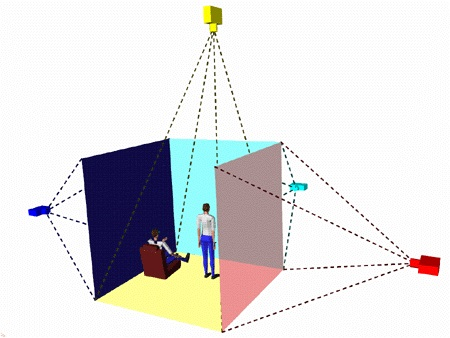
\includegraphics[scale=0.9]{graphic/cave2_pogladowy}
\par\end{centering}
\caption{Wyświetlanie obrazu w CAVE\protect \\
Źródło: http://escience.anu.edu.au/lecture/cg/Display/cave.en.html
(dostęp: 07.05.2016)}

\end{figure}

Ilustracja załączona powyżej przedstawia podstawowe założenia budowy
środowiska jaskini wirtualnej rzeczywistości. W standardowy rozkład
ścian wchodzi: przednia, boczne oraz podłogowa. Projektory umieszczone
są na zewnątrz, rzucając obraz od tyłu – jest to tzw. tylna projekcja
(ang: Rear Screen Projection). Obraz rzucany na podłogę może być przez
projektor z góry lub z dołu. Projektory użyte do wyświetlania muszą
charakteryzować się wysoką rozdzielczością oraz szybkim odświeżaniem.
Zazwyczaj jest to rozdzielczość FullHD oraz odświeżanie o częstotliwości
powyżej 90Hz. Obraz rzucany na kwadratową ścianę jest ucinany na bokach
a Często wykorzystuje się lustra by zmniejszyć odległość między projektorem
a ekranem. Każdy projektor jest kontrolowany przez jeden z komputerów
połączonych w klaster. W klastrze jeden z komputerów jest nadrzędny
i sprawuje kontrole nad pozostałymi, renderującymi obraz dla projektorów.
Jest to rozwiązanie zwiększające szybkość generowania klatek oraz
tańsze w utrzymaniu.

Obraz wyświetlany w jaskini wirtualnej jest dostosowywany zależnie
od położenia „użytkownika głównego”. Kamery śledzą położenie czujników
zamontowanych na okularach by wyświetlany obraz był odpowiednio zsynchronizowany
na krawędziach i dopasowany do perspektywy odbiorcy. Każdy inny użytkownik,
który nie jest śledzony przez kamery widzi obraz nieco przesunięty
względem użytkownika głównego. Objawia się to źle sklejonym obrazem
lub/i nienaturalną perspektywą.

\begin{figure}[H]
\begin{centering}
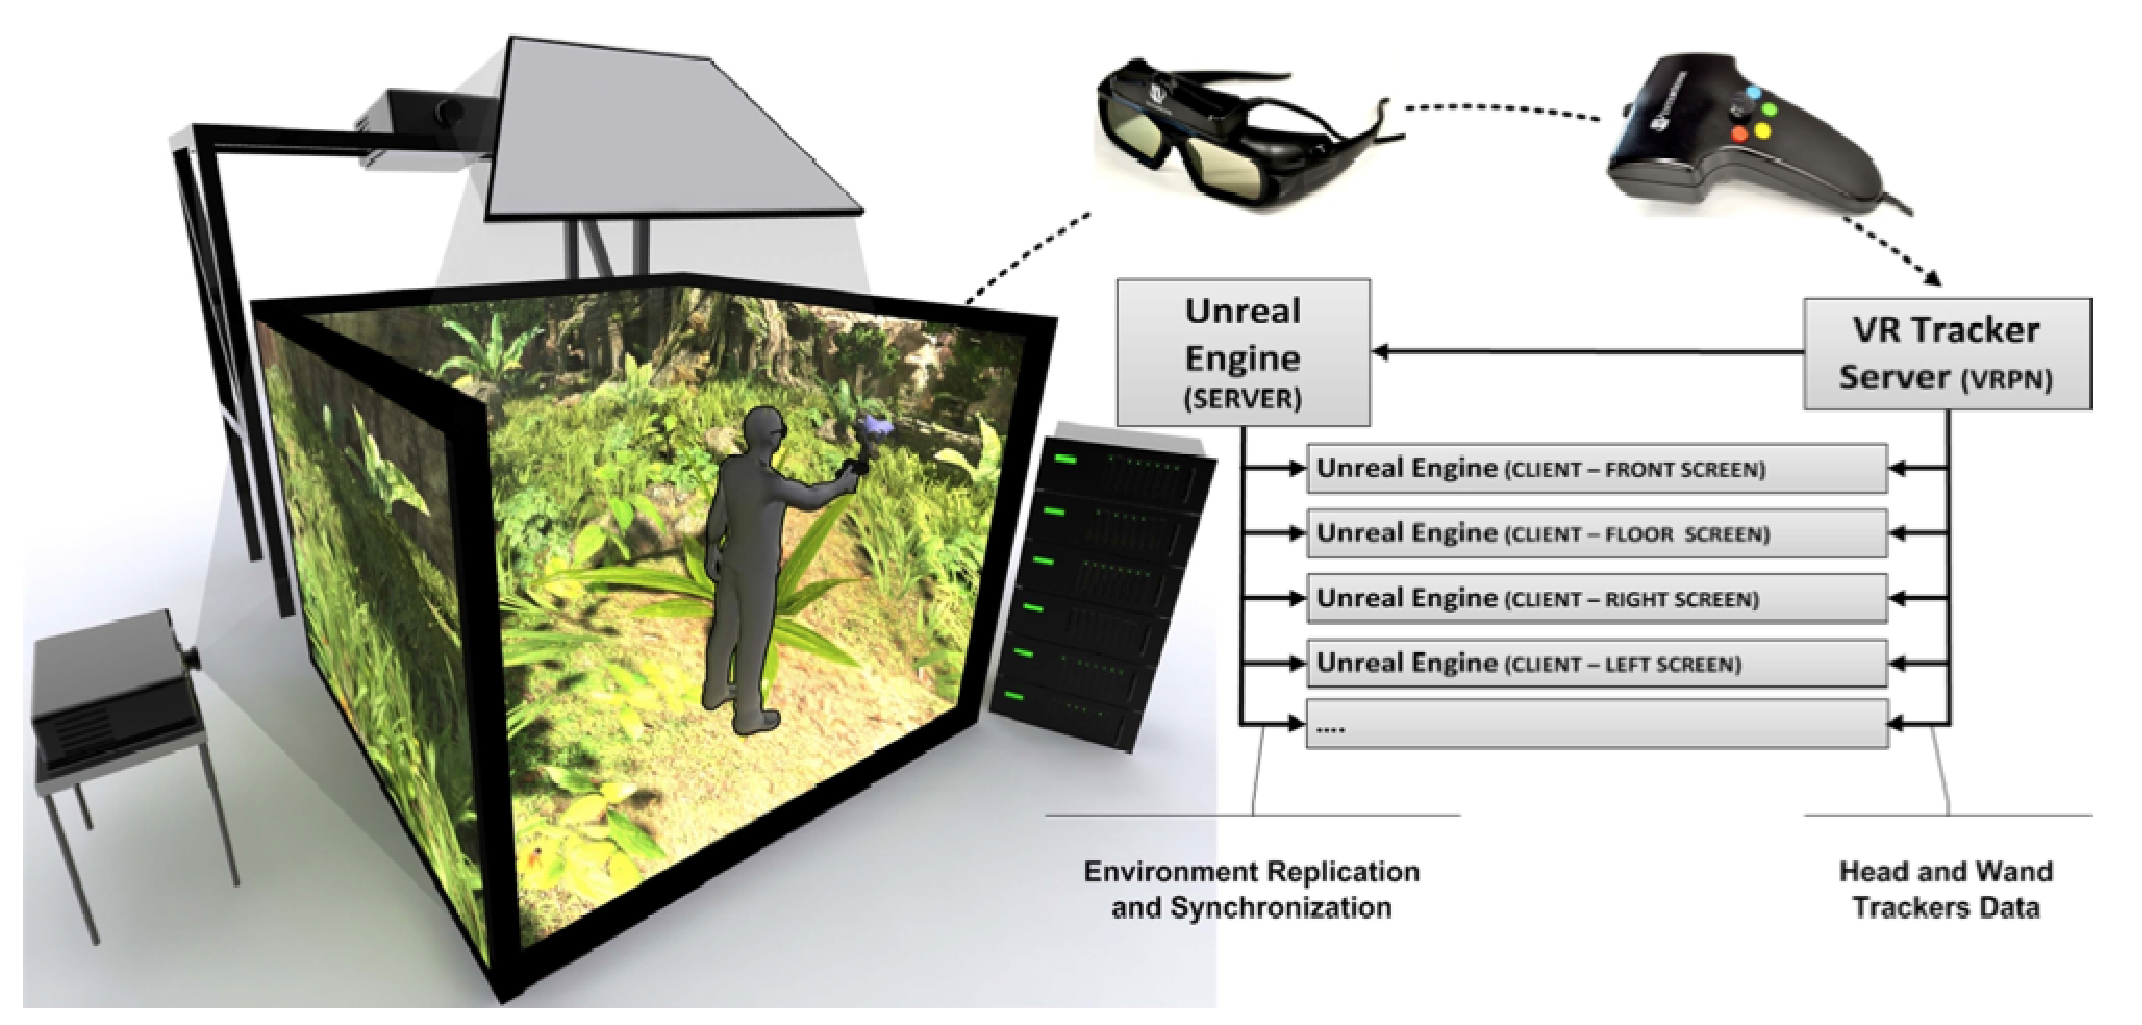
\includegraphics[scale=0.4]{graphic/CaveUDK_Architecture}
\par\end{centering}
\caption{Architektura systemu CAVE na przykładzie użycia Unreal Engine}

\end{figure}

Oprócz samego wyświetlania obrazu, jaskinia wirtualnej rzeczywistości
pozwala również na interakcje ze światem otaczającym. Dzieje się to
przy pomocy różnych kontrolerów np. FlySticka lub MagicWand. Są to
bezprzewodowe joysticki wyposażone w zestaw czujników potrafiących
określić pozycje (jako zestaw trzech wektorów) oraz orientacje (podawaną
jako kwaternion) urządzenia w przestrzeni. Oprócz tego kontroler wyposażony
jest w podstawowe części takie jak: analogowy, dwuosiowy joystick
oraz kilka przycisków i/lub trigger. Przykładowy model został pokazany
na obrazku (Fig. 3).

\begin{figure}[H]
\begin{centering}
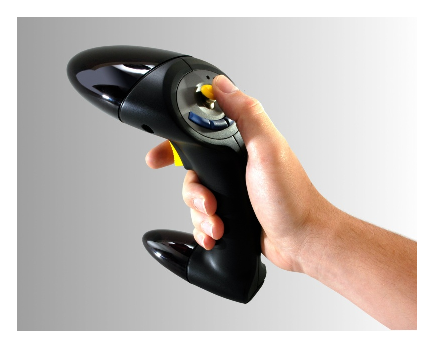
\includegraphics[scale=0.8]{graphic/Flystick_2small}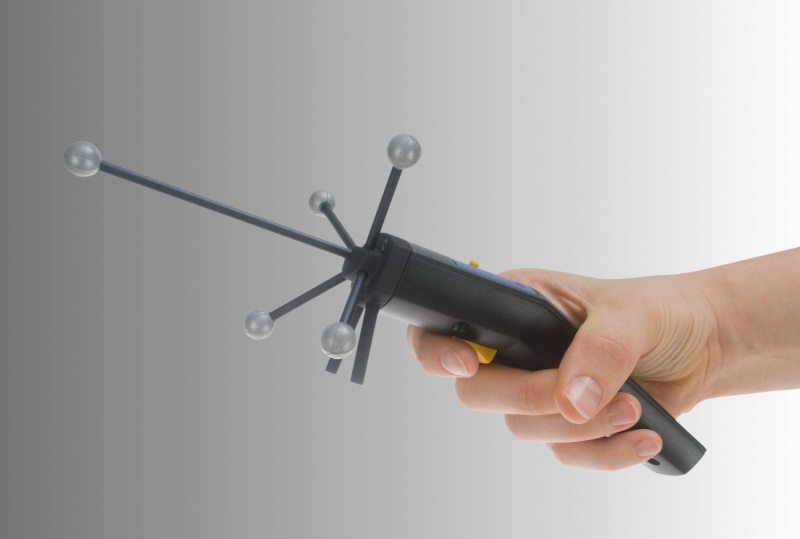
\includegraphics[scale=0.8]{graphic/Flystick3_small}\caption{Dwa modele joysticka Flystick firmy ART\protect \\
Źródło: http://www.middlevr.com/doc/1.2/ch04s03.html (dostęp 07.05.2016)}
\par\end{centering}
\end{figure}


\subsection{Porównanie HMD i CAVE\protect\footnote{http://www.visbox.com/technology/cave-vs-hmd/ (dostęp 07.05.20016)}}

Head-mounted display oraz CAVE to bardzo różniące się sposoby na wizualizację
świata wirtualnego. Wysokie koszty jaskini wirtualnej rzeczywistości
pozwalają na większe możliwości wykorzystania oraz trochę większy
komfort użytkowania. Z drugiej strony jednak jaskinia wirtualnej rzeczywistości
zajmuje bardzo dużo miejsca w porównaniu do okularów wirtualnej rzeczywistości,
które są też o wiele tańsze.

\begin{table}[H]
\begin{centering}
\caption{Porównanie HMD i CAVE\protect \\
Źródło: Opracowanie własne, http://www.visbox.com/technology/cave-vs-hmd/}
\par\end{centering}
\centering{}%
\begin{tabular*}{15cm}{@{\extracolsep{\fill}}|>{\centering}p{3cm}|>{\centering}p{4cm}|>{\centering}p{5cm}|}
\cline{2-3} 
\multicolumn{1}{>{\centering}p{3cm}|}{} & HMD & CAVE\tabularnewline
\hline 
Rozdzielczość (w megapikselach) & 1-2 Mpx/oko & 2-8 Mpx/ekran\tabularnewline
\hline 
Jakość obrazu & Wymaga użycia zniekształcenia; dobra & bardzo dobra\tabularnewline
\hline 
Immersja & Bardzo duża & Duża\tabularnewline
\hline 
Pole widzenia (w stopniach) & \textasciitilde{}110 & Takie jak człowieka\tabularnewline
\hline 
Mobilność użytkownika & Ograniczona okablowaniem i czujnikami & Nieograniczona\tabularnewline
\hline 
Użytkownicy & Jeden & Wielu\tabularnewline
\hline 
Komfort użytkowania & Ekran blisko oka może wywoływać ból głowy; możliwe nudności & Ekrany daleko od oka co pozwala na dłuższe użytkowanie; możliwe nudności\tabularnewline
\hline 
Koszt & Niewielki & Wysoki\tabularnewline
\hline 
\end{tabular*}
\end{table}

Obecnie systemy wirtualnej jaskini ją wykorzystywane głównie w laboratoriach
instytutów. Nie są one dostępne dla szerszego odbioru. Urządzenia
HMD są za to dostępne dla każdego a~ich obsługa i ustawienie jest
znacznie łatwiejsze. Na rynku pojawiają się również coraz więcej modeli
znanych i mniej znanych firm przystosowanych specjalnie do smartfonów.
Wybór wśród nich jest więc znacznie wiekszy niż w przypadku CAVE'ów,
które często muszą instalować i częściowo obsługiwać zewnętrzne firmy.

\section{Opis aplikacji BlenderVR}

\subsection{Opis aplikacji\protect\footnote{Strona instytutu LIMSI we Francji https://blendervr.limsi.fr/doku.php
(dostęp 07.05.20016)}}

Aplikacja BlenderVR powstała w laboratorium LIMSI we Francji. Twórcami
są: Dalai Felinto, Damien Touraine, David Poirier-Quinot, Laurent
Pointal i Bran F.G. Katz. Aplikacja pozwala na użycie scen generowanych
przez Blender Game Engine, w środowiskach wirtualnych: CAVE, okulary
wirtualnej rzeczywistości HMD lub Video Wall.

BlenderVR jest narzędziem skalowalnym oraz wieloplatformowym. Działa
zarówno na komputerach z system Windows jak i Linux/iOS. Przenoszenie
sceny pomiędzy różnymi platformami wirtualnej rzeczywistości nie wymaga
jej edytowania. Wszystkim zajmuje się odpowiednia konfiguracja programu.
Aplikację można dostosować do dowolnej liczby komputerów obsługujących
różne ekrany. BlenderVR posiada wsparcie dla wyświetlania obrazu 3D
(poczwórne buforowanie - ang: Quad Buffering) i protokołów komunikacyjnych
np. VRPN – virtual reality peripherial network lub OSC – open sound
control.

\begin{figure}[H]
\begin{centering}
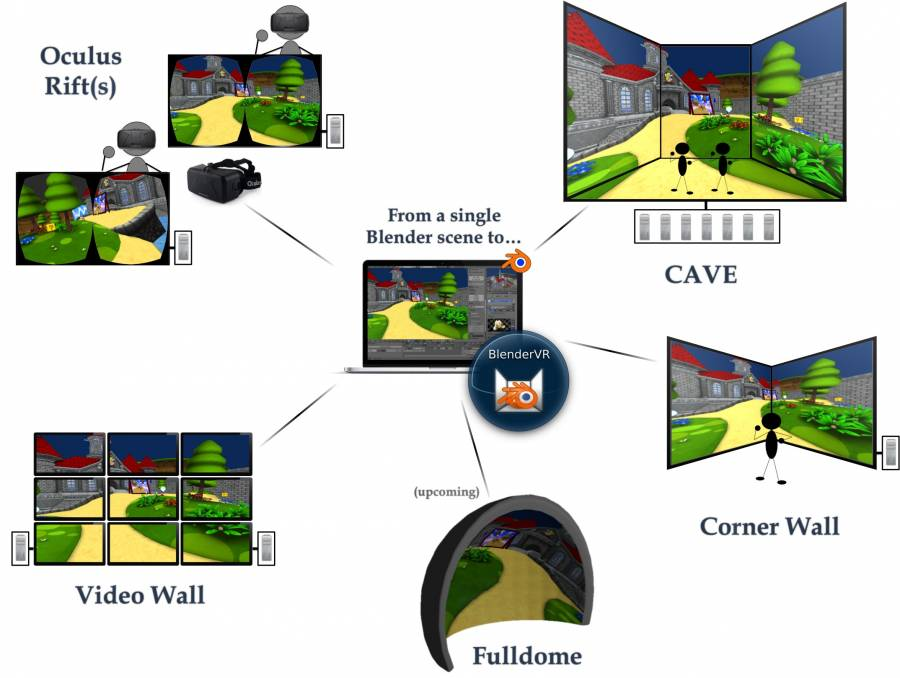
\includegraphics[scale=0.4]{graphic/blendervr-applications}
\par\end{centering}
\caption{Możliwości i zastosowania aplikacji BlenderVR\protect \\
Źródło: https://blendervr.limsi.fr/doku.php (dostęp 07.05.20016)}
\end{figure}

Wszystkie ustawienia BlenderVR znajdują się w jednym pliku XML. Ułatwia
to przenoszenie konfiguracji pomiędzy komputerami lub jej klonowanie.
W pliku konfiguracyjnym najważniejszymi ustawieniami są:
\begin{itemize}
\item Ścieżki do bibliotek i programów, z których korzysta BlenderVR.
\item Adresy komputerów typu „slave” – obsługujących wyświetlanie obrazu
oraz dane logowania przez protokół SSH.
\item Ilość ekranów, ich położenie oraz relacje oko - ekran.
\item Ustawienia wtyczki do interakcji ze sceną: serwer odbierający dane
z urządzeń wskazujących oraz konfiguracja czujników.
\end{itemize}
Interfejs jest przejrzysty i prosty w obsłudze. Po uruchomieniu wystarczy
załadować odpowiedni plik konfiguracyjny, następnie wybrać konfigurację
ekranów i wskazać miejsca pliku ze sceną do symulacji. W zakładce
„Run” znajduje się przycisk do uruchomienia programu oraz konsola
do debugowania.

\begin{figure}[H]
\begin{centering}
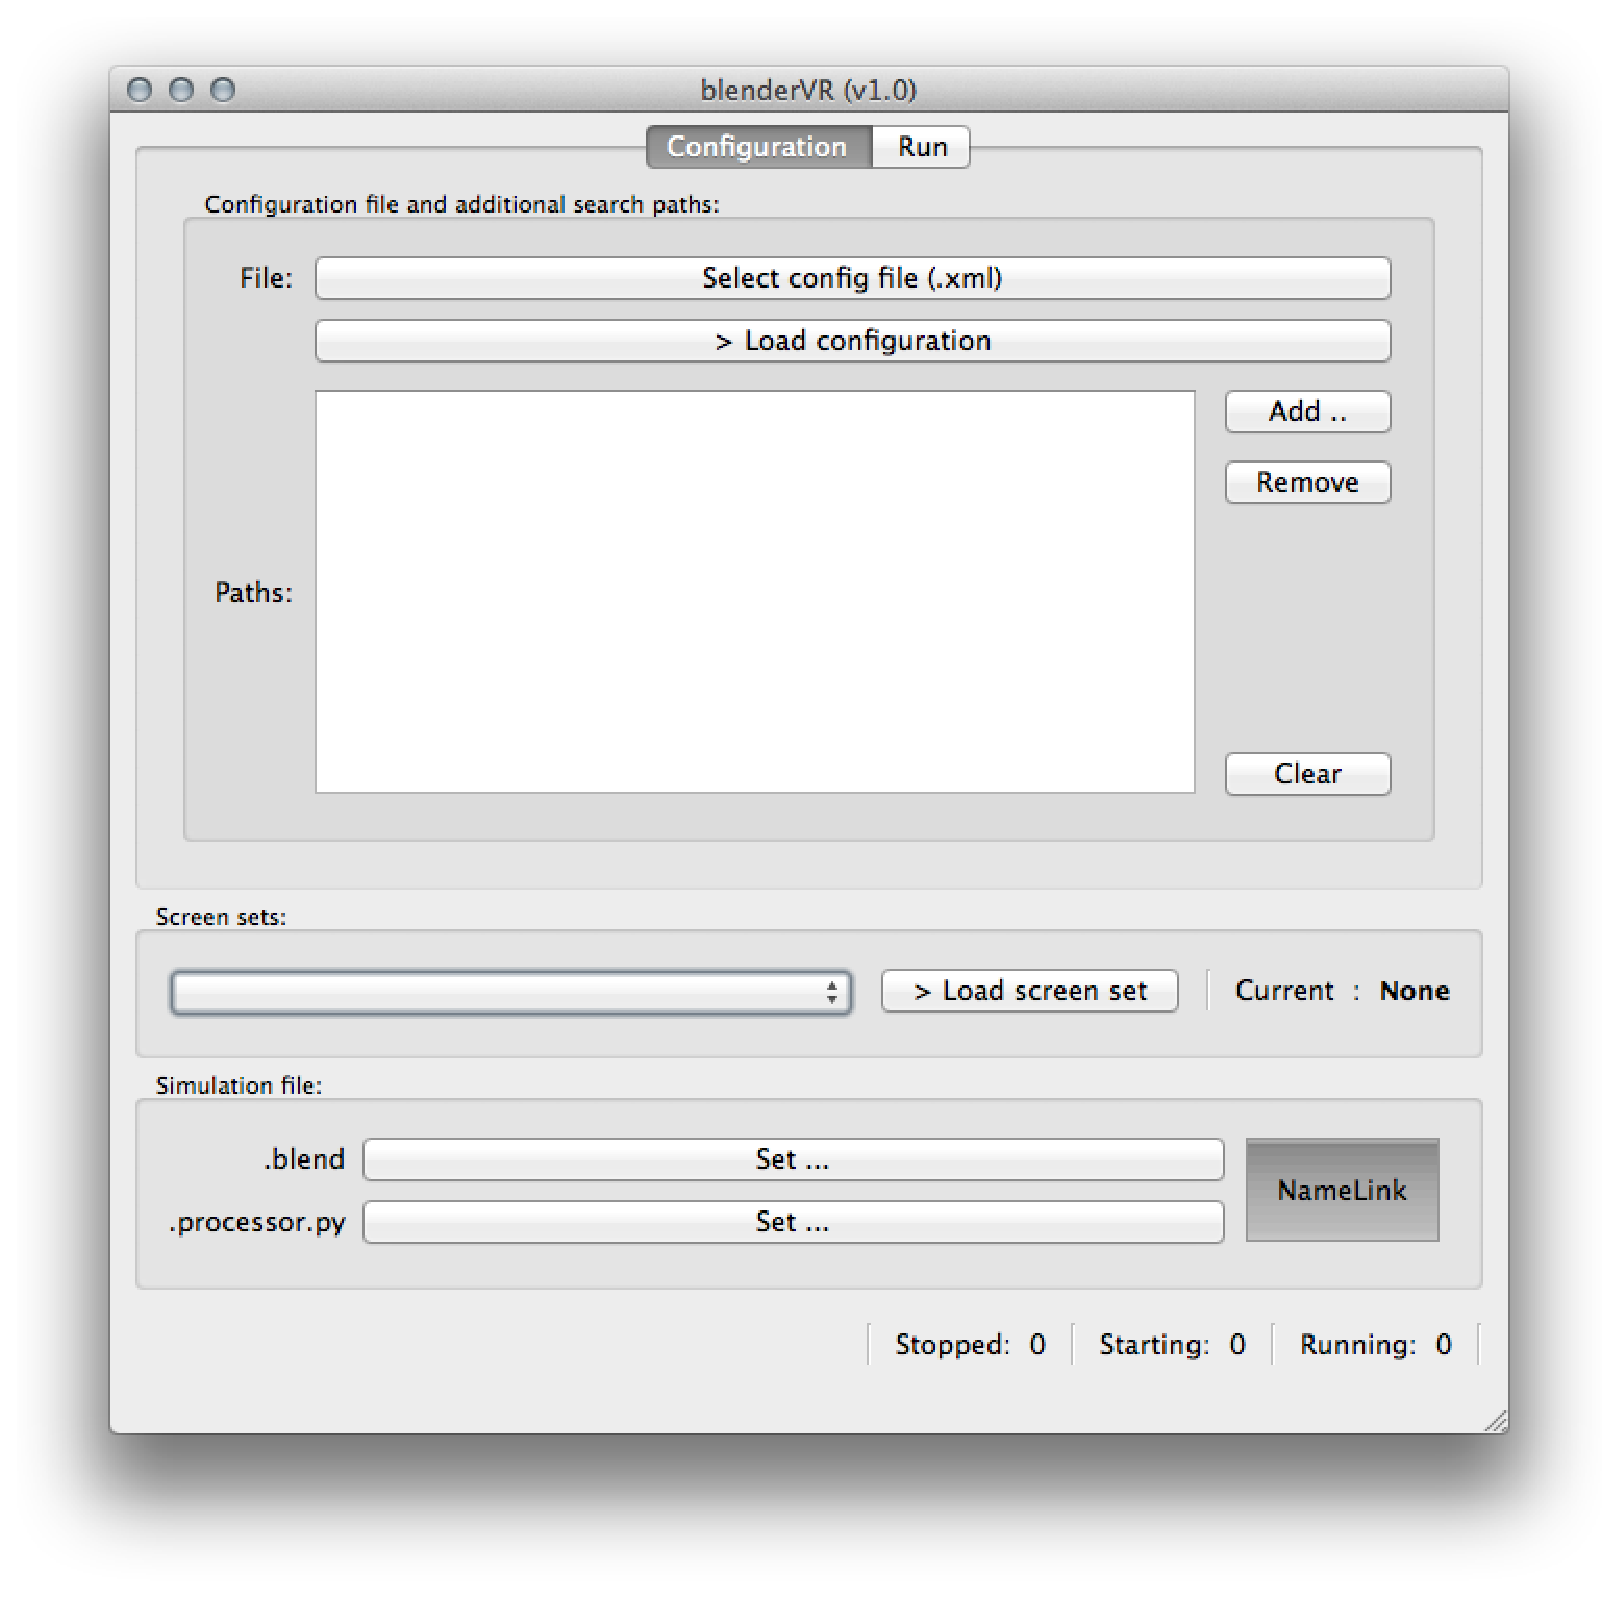
\includegraphics[scale=0.4]{graphic/user-interface-1}
\par\end{centering}
\caption{Interfejs aplikacji BlenderVR\protect \\
Źródło: https://blendervr.limsi.fr/doku.php (dostęp 07.05.20016)}
\end{figure}


\subsection{Opis pliku konfiguracyjnego}

Jedną z najwazniejszych części aplikacji jest plik konfiguracyjny.
W nim zawarte są wszystkie informacje odnośnie połączeń do komputerów
podrzędnych, ustawień ekranów, wyświetlania obrazu oraz konfiguracji
wtyczek. Plik ustawień zapisywany jest w formacie XML. Ułatwia to
edycję ponieważ wystarczy do tego zwykły edytor plików tekstowych.
Przykładowa konfiguracja dla CAVE w systemie Linux:

<?xml version="1.0"?>
<blendervr>
  <starter anchor='/tmp/console' blender='/usr/local/blender/2.74/bin/blender'>
     <config name='console'>console screen</config>
     <config name='virtual environment'>console screen, front screen, left screen, right screen
</config>
  </starter>
  <users>
<user name='user A' />
  </users>
  <!-- Here, we define the console parameters -->
  <computers>
    <computer name='console computer' hostname='console.fqdn'/>
  </computers>
  <screens>
    <screen name='console screen' computer='console computer'>
      <display options='-w 600 600'>
  <environment>DISPLAY=:0.0</environment>
  <graphic_buffer user='user A'/>
      </display>
      <wall>
  <corner name='topRightCorner'>1.0, 1.0, -1.0</corner>
  <corner name='topLeftCorner'>-1.0, 1.0, -1.0</corner>
  <corner name='bottomRightCorner'>1.0, -1.0, -1.0</corner>
      </wall>
    </screen>
  </screens>
  <computers>
    <system root='/usr/local/blender/vr/1.0' anchor='/tmp/node'>
      <login remote_command="ssh `self._attributs_inheritance['hostname']`"
python='/usr/local/blender/2.74/dependencies/bin/python3.3'/>
      <daemon transmit='True'>   <environment>PATH=/usr/bin:/bin</environment>
      </daemon>
      <blenderplayer executable='/usr/local/blender/2.74/bin/blenderplayer' />
    </system>
    <computer name='front computer' hostname='front.fqdn' />
    <computer name='right computer' hostname='right.fqdn' />
    <computer name='left computer' hostname='left.fqdn' />
  </computers>
  <screens>
    <display options='-f -s hwpageflip'>
      <environment>DISPLAY=:0.0</environment>
      <graphic_buffer buffer='left' user='user A' eye='left'/>
      <graphic_buffer buffer='right' user='user A' eye='right'/>
    </display>
    <screen name='front screen' computer='front computer'>
      <wall>
  <corner name='topRightCorner'>1.0, 1.0, -1.0</corner>
  <corner name='topLeftCorner'>-1.0, 1.0, -1.0</corner>
  <corner name='bottomRightCorner'>1.0, -1.0, -1.0</corner>
      </wall>
    </screen>
    <screen name='left screen' computer='left computer'>
      <wall>
  <corner name='topRightCorner'>-1.0, 1.0, -1.0</corner>
  <corner name='topLeftCorner'>-1.0, 1.0, 1.0</corner>
  <corner name='bottomRightCorner'>-1.0, -1.0, -1.0</corner>
      </wall>
    </screen>
    <screen name='right screen' computer='right computer'>
      <wall>
  <corner name='topRightCorner'>1.0, 1.0, 1.0</corner>
  <corner name='topLeftCorner'>1.0, 1.0, -1.0</corner>
  <corner name='bottomRightCorner'>1.0, -1.0, 1.0</corner>
      </wall>
    </screen>
</screens>
  <plugins>
<vrpn>
<floor x='0.0'/>
      <tracker device='GTK' host='localhost'>
  <transformation>
    <post_translation z='-1.6'/>
    <post_rotation x='1.0' y='1.0' z='1.0' angle="`-2*math.pi/3`"/>
    <pre_rotation x='1.0' y='1.0' z='1.0' angle="`2*math.pi/3`"/>
  </transformation>
  <sensor id='0' processor_method='user_position' users='user A'/>
  <sensor id='1' processor_method='tracker_1'/>
  <sensor id='2' processor_method='tracker_2'/>
  <sensor id='3' processor_method='tracker_3'/>
      </tracker>
      <analog device='GTK' host='localhost' processor_method='movements'/>
      <button device='GTK' host='localhost' processor_method='buttons'/>
    </vrpn>
  </plugins>
</blendervr>

\subsubsection*{Sekcja <Starter>}

Zawiera definicje ustawień ekranów. Lista musi zawierać wszystkie
ekrany oddzielone przecinkami, które będą używane w danej formie ustawienia.
Np. ustawienie,,console'' będzie korzystać tylko z ekranu o nazwie,,console''
natomiast ustawienie,,CAVE'' z ekranów: floor, front, left, right.
Sekcja wskazuje również gdzie znaleźć program Blender3D.

\subsubsection*{Sekcja <Users>}

Każdy użytkownik, który będzie śledzony powinien zostać tutaj wpisany.
Dzięki temu program dostosuje renderowany obraz do położenia danego
użytkownika. Dla każdego z wpisanych użytkowników należy zdefiniować
pozycję startową (default\_position) oraz rozstaw oczu (eye\_separation).

\subsubsection*{Sekcja <Computers>}

W tej sekcji opisany jest jak każdy z komputerów renderujących działa.
Mieszczą się tutaj informacje odnośnie konfiguracji blenderplayer
np. ścieżki do plików, zmienne środowiskowe itp. Mogą być one różne
dla każdego stanowiska. Każdy węzeł renderujący (komputer) musi mieć
sprecyzowaną nazwę oraz adres sieciowy (lub nazwę sięciową).

\subsubsection*{Sekcja <System>}

Zawiera ścieżki do najważniejszych plików programu oraz systemu, zwłaszcza
w przypadku platformy Windows gdzie należy podać ścieżkę do katalogu
Windowsa. Tutaj można dopisywać również ścieżki wspólne dla wszystkich
stacji renderujących. Jeśli pewne ścieżki na każdym z komputerów są
takie same wystarczy umieścić je tutaj zamiast wypisywać to samo dla
każdego komputera w sekcji <computers>. Sekcja ta zawiera kilka szczególnych
podsekcji, które warto opisać:
\begin{itemize}
\item Library Path - pluginy często wymagają dostępu do zewnętrznych bibliotek.
W tej podsekcji możemy wskazać gdzie znajdują się niezbędne pliki.
Np: \texttt{<library path=\textquotedbl{}/usr/local/lib/vrpn/\textquotedbl{}
/>}.
\item Login - precyzuje jak wygląda komenda połączenia się z komputerami
odpowiedzialnymi za renderowanie. Np: \texttt{<login remote\_command=\textquotedbl{}ssh
me@host\textquotedbl{} python=\textquotedbl{}/usr/bin/python3\textquotedbl{}/>}.
\item Daemon - opcje dotyczące uruchomienia demona. Parametr \textbf{Transmit}
decyduje czy demon przesyła zmienne środowiskowe do blendera kiedy
go uruchamia. \textbf{Environment} natomiast dodaje specyficzne zmienne
środowiskowe dla samego demona.
\item Blenderplayer - w tej podsekcji ustawiona jest ścieżka do aplikacji
blenderplayer.
\end{itemize}

\section{Instalacja i testy aplikacji w Laboratorium Zanurzonej Wizualizacji
Przestrzennej}

\subsection{Środowisko wdrożeniowe systemu Windows}

Test aplikacji BlenderVR został przeprowadzony na specjalnie przygotowanych
stanowiskach komputerowych. W skład jednostki testowej wchodził sprzęt:
\begin{itemize}
\item Komputer stacjonarny wyposażony w:

\begin{itemize}
\item procesor Intel Xeon E5-1630
\item karta graficzna Nvidia Quadro k5200
\item 32 GB pamięci RAM
\item Dysk HDD o pojemności 500 GB
\end{itemize}
\item Monitor ASUS 24'' z możliwością wyświetlenia obrazu 3D. Częstotliwość
odświeżania do 144Hz
\item Aktywne okulary 3D
\end{itemize}
System operacyjny zainstalowany na jednostkach testowych to Windows
7 Professional. Każdy komputer wpięty został w tę samą sieć Ethernet.
Żaden nie ma dostępu do Internetu. Wszystkie niezbędne programy oraz
pakiety zostały dostarczone ze źródeł zewnętrznych przy użyciu dysku
przenośnego.

\subsection{Instalacja aplikacji BlenderVR w systemie operacyjnym Windows}

Deweloperzy dostarczają gotową paczkę instalacyjną. Należy ściągnąć
instalator ze strony internetowej oraz go uruchomić. Podczas procesu
oprócz BlenderVR zostanie zainstalowany również Python oraz pakiet
bibliotek graficznych Qt4.8. W systemie dodatkowo zostaną utworzone
ścieżki tak, by aplikacja przy uruchomieniu nie miała problemów ze
znalezieniem wszystkich zależności. W laboratorium instalacja paczki
BlenderVR przebiegła pomyślnie i bez żadnych problemów.

\subsection{Uruchomienie aplikacji BlenderVR w systemie operacyjnym Windows}

W przypadku systemu operacyjnego Windows uruchomienie jest proste.
Wystarczy użyć skrótu na pulpicie, który jest tworzony po zainstalowaniu
gotowej paczki. Przygotowano odpowiedni plik konfiguracyjny dla systemu
Windows na bazie przykładu dostępnego na stronie dewelopera: 

<?xml version=\textquotedbl{}1.0\textquotedbl{}?> 

	<blendervr>     

	 <starter blender=\textquotedbl{}C:/blender/blender.exe\textquotedbl{}> 

<config name=\textquotedbl{}Fullscreen\textquotedbl{}>fullscreen</config>
  

<config name=\textquotedbl{}Console\textquotedbl{}>console</config>
      

	<config name=\textquotedbl{}Split\textquotedbl{}>console half left,
console half right</config>   

</starter>  

<users> 

<user name=\textquotedbl{}user A\textquotedbl{} />  

</users>   

<computers>   

<system> 

<daemon transmit=\textquotedbl{}True\textquotedbl{}>

<environment>SystemRoot=C:/Windows</environment>

</daemon>   

<blenderplayer executable=\textquotedbl{}C:/blender/blenderplayer.exe\textquotedbl{}
/>

</system>  

      <computer name=\textquotedbl{}Any\textquotedbl{} hostname=\textquotedbl{}{*}\textquotedbl{}
/> 

   </computers>  

  <screens>    

    <screen name=\textquotedbl{}fullscreen\textquotedbl{} computer=\textquotedbl{}Any\textquotedbl{}>
 

           <display options=\textquotedbl{}-f\textquotedbl{}> 

           <graphic\_buffer buffer=\textquotedbl{}mono\textquotedbl{}
user=\textquotedbl{}user A\textquotedbl{} eye=\textquotedbl{}middle\textquotedbl{}
/>

           </display>  

          <wall>   

             <corner name=\textquotedbl{}topRightCorner\textquotedbl{}>1.0,
1.0, -1.0</corner> 

             <corner name=\textquotedbl{}topLeftCorner\textquotedbl{}>-1.0,
1.0, -1.0</corner> 

             <corner name=\textquotedbl{}bottomRightCorner\textquotedbl{}>1.0,
-1.0, -1.0</corner> 

           </wall>     

   </screen>    

   <screen name=\textquotedbl{}console\textquotedbl{} computer=\textquotedbl{}Any\textquotedbl{}>
   

      	 <display options=\textquotedbl{}-w 400 400\textquotedbl{}> 

           <graphic\_buffer buffer=\textquotedbl{}mono\textquotedbl{}
user=\textquotedbl{}user A\textquotedbl{} eye=\textquotedbl{}middle\textquotedbl{}
/>

           </display>   

         <wall>        

        <corner name=\textquotedbl{}topRightCorner\textquotedbl{}>1.0,
1.0, -1.0</corner>  

             <corner name=\textquotedbl{}topLeftCorner\textquotedbl{}>-1.0,
1.0, -1.0</corner>   

             <corner name=\textquotedbl{}bottomRightCorner\textquotedbl{}>1.0,
-1.0, -1.0</corner>  

          </wall>   

     </screen>   

     <screen name=\textquotedbl{}console half left\textquotedbl{}
computer=\textquotedbl{}Any\textquotedbl{}> 

           <display options=\textquotedbl{}-w 400 400 200 300\textquotedbl{}>

            <graphic\_buffer user=\textquotedbl{}user A\textquotedbl{}
/>

            </display>

            <wall>

                <corner name=\textquotedbl{}topRightCorner\textquotedbl{}>0.0,
1.0, -1.0</corner>

                <corner name=\textquotedbl{}topLeftCorner\textquotedbl{}>-1.0,
1.0, -1.0</corner>

                <corner name=\textquotedbl{}bottomRightCorner\textquotedbl{}>0.0,
-1.0, -1.0</corner>

            </wall>

      </screen>

      <screen name=\textquotedbl{}console half right\textquotedbl{}
computer=\textquotedbl{}Any\textquotedbl{}>

            <display options=\textquotedbl{}-w 400 400 600 300\textquotedbl{}>

                <graphic\_buffer user=\textquotedbl{}user A\textquotedbl{}
/>

            </display>

            <wall>

                <corner name=\textquotedbl{}topRightCorner\textquotedbl{}>1.0,
1.0, -1.0</corner>

                <corner name=\textquotedbl{}topLeftCorner\textquotedbl{}>0.0,
1.0, -1.0</corner>

                <corner name=\textquotedbl{}bottomRightCorner\textquotedbl{}>1.0,
-1.0, -1.0</corner>

            </wall>

</screen>

    </screens>

    <plugins></plugins>

</blendervr>

Po pierwszej próbie uruchomienia BlenderVR konsola systemu Windows
zwróciła błąd: \texttt{C:\textbackslash{}BlenderVR\textbackslash{}Required\textbackslash{}Python3\textbackslash{}python.exe: Can't
open file C:/BlenderVR/source/utilsdaemon.py}. Natomiast okienko logowania
BlenderVR wyświetliło komendę, która była wykonywana przy ładowaniu
pliku: \texttt{C:/BlenderVR/Required/Python3/python.exe C:/BlenderVR/source/utils\textbackslash{}daemon.py}.
Wiersz tekstu w pliku konfiguracyjnym odpowiedzialny za początek ścieżki:
\texttt{<system root='C:/BlenderVR/source/'>} oraz za wykonanie polecenia
uruchomienia skryptu: \texttt{C:/BlenderVR/Required/Python3/python.exe}.
Wyglądało na to, że aplikacja dodaje do ścieżki katalog oraz skrypt
do uruchomienia jednak z błędnym znakiem separacji katalogów. Zwrócono
uwagę na to, że program nie parsuje wszystkich ścieżek odpowiednio
do systemu operacyjnego. W systemach Windows używany jest znak '\textbackslash{}'
jako separator katalogów. W przykładowym pliku konfiguracyjnym na
stronie dewelopera (na podstawie którego pisany był plik aktualnie
testowany) znajdują się ścieżki pisane w stylu unixowym. Zmiana znaków
w pliku konfiguracyjnym ze \textquotedbl{}slash\textquotedbl{} na
\textquotedbl{}backslash\textquotedbl{} spowodowała inny błąd. Tym
razem w oknie logowania wyświetlone zostało \texttt{C:BlenderVRRequiredPython3Python.exe
command not found}. Zdiagnozowano dzięki temu problem z parsowaniem
znaków '/' i '\textbackslash{}' przez aplikację.

Moduł odpowiedzialny za ładowanie demona został znaleziony w pliku:
\texttt{BlenderVR/modules/blendervr/console/logic/screen.py}. Fragment
kodu: \texttt{self.\_daemon{[}'command'{]}.append(os.path.join(system{[}'root'{]},'utils',
'daemon.py')).} Za przygotowanie ścieżki odpowiedniej dla danego systemu
odpowiedzialna jest część \texttt{os.path.join}. W przypadku systemu
Windows komenda ta dostawia ‘\textbackslash{}’ do ścieżki, co powodowało
błąd przy dalszym parsowaniu ścieżki. Z powyższych testów wynikało
jednak, że dostawiony backslash jest błędny i usuwany podczas przekazywania
komendy do konsoli Windowsa. Zmieniono tą część kodu i wpisano na
sztywno: \texttt{self.\_daemon{[}'command'{]}.append(\textquotedbl{}/\textquotedbl{}.join((system{[}'root'{]},
utils', 'daemon.py'))).} Poprawka w kodzie pozwoliła aplikacji odpowiednio
zinterpretować ścieżki. Do konsoli Windows została przekazana następująca
komenda: \texttt{C:/BlenderVR/Required/Python3/python.exe C:/BlenderVR/source/utils/daemon.py}.
Wpis w okienku logowania „Daemon for screen console started” oznajmił,
że konfiguracja jest prawidłowa i załadowana. Następnie wybrano jedną
z dostępnych scen przykładowych. Załadowano ją wraz z odpowiadającym
jej plikiem procesora dla sceny. Po przejściu do zakładki „run” i
kliknięciu przycisku startu na ekranie pojawiła się wybrana scena.
Próba uruchomienia w podstawowej konfiguracji zakończyła się sukcesem. 

\subsubsection{Testy z wykorzystaniem dwóch stanowisk PC}

Środowisko jaskini wirtualnej rzeczywistości wymaga współpracy kilku
stanowisk komputerowych. W tym celu każde z nich musi zostać wyposażone
w aplikację pokazującą obraz z perspektywy danego urządzenia wyświetlającego.
BlenderVR wykorzystując protokół SSH potrafi zarządzać swoimi kopiami
na komputerach typu ,,slave''. Jeden komputer zdefiniowany jako
nadrzędny,,master'' może uruchamiać oraz synchronizować inne instancje
BlenderVR na komputerach typu ,,slave''.

Na tej zasadzie jedno ze stanowisk w laboratorium stało się nadrzędne
względem drugiego stanowiska -,,slave'a''. Na obu komputerach zainstalowano
w ten sam sposób aplikację BlenderVR. Niestety system operacyjny Windows
nie posiada wbudowanego protokołu SSH. Program OpenSSH for Windows
pozwolił na uzyskanie bezpośredniego połącznia przez ten protokół.
Między komputerami wymieniono klucze do identyfikacji. Pozwoliło to
na połączenie nie wymagające hasła. Jest to jeden z wymogów aplikacji
BlenderVR do jej poprawnego działania.

W przypadku połączenia między wieloma komputerami należy w plik konfiguracyjny
wpisać każdy z komputerów podrzędnych. W sekcji <computers> każda
z wpisanych jednostek powinna zawierać:
\begin{itemize}
\item Nazwę własną
\item Adres IP w sieci
\item Ścieżkę do katalogu głównego aplikacji BlenderVR
\item Ścieżkę do katalogu z przykładowymi scenami
\item Ścieżkę do głównego katalogu systemu (w tym przypadku do katalogu
Windows)
\item Ścieżkę do BlenderPlayer z Blendera3D
\end{itemize}
BlenderVR przy połączeniu do drugiego stanowiska próbuje uruchomić
na nim skrypt,,demona'' - programu działającego w tle, który cały
czas przetwarza dane lub wykonuje pewne czynności\footnote{http://www.python.rk.edu.pl/w/p/proste-demony-uniksowe-w-pythonie/
(dostęp: 16.06.2016)}. Odpowiednio zapisany plik konfiguracyjny został załadowany do aplikacji.
Niestety konsola z informacjami wyświetliła błąd,,Error: Cannot start
daemon for screen <screenName>''. Na stronie BlenderVR błąd jest
rozpoznany i według autora rozwiązania problem występuje jeśli połączenie
miedzy komputerami wymaga hasła. Błąd w tym przypadku nie powinien
występować ponieważ komputery zostały wymienione kluczami. Połączenie
SSH zostało przetestowane poprzez konsolę Windowsa i nie wymagało
użycia hasła. Po konsultacji jeden z twórców oprogramowania polecił
sprawdzić czy polecenie wykonywane przez BlenderVR można również wykonać
ręcznie przez konsolę. Ręczne wykonanie nie zwróciło jednak żadnego
błędu; komenda wykonała się poprawnie.

Problemem w tym przypadku może być konfiguracja serwera SSH, które
nie pozwala na logowanie jako administrator. Logowanie przez protokół
na komputer podrzędny odbywało się przy użyciu konta z prawami administratora.
Zanim stanowiska zostały wymienione kluczami, do logowania było wymagane
hasło takie samo jak przy logowaniu użytkownika na docelowym systemie.
Teoretycznie rzecz biorąc po zalogowaniu się przez SSH, użytkownik
powinien mieć wszystkie niezbędne prawa do zarządzania komputerem.

Kolejną możliwością jest brak praw administratorskich środowiska Python.
Skrypt wykonywany przez aplikację BlenderVR wymaga uruchomienia najpierw
Pythona a później skryptu demona. Być może uruchamia się on bez praw
administratora co nie pozwala mu na działanie w tle.

<tutaj coś jeszcze rozwinąć>

\subsection{Krótki test w środowisku Linux <\textcompwordmark{}<lub 4.0 jako
kolejny rozdział>\textcompwordmark{}>}

Powyższe próby implenetacji oraz uruchomienia aplikacji BlenderVR
pokazały, że nie jest on w pełni dostosowany do systemu operacyjnego
jakim jest Windows. Brak najprostszych protokołów komunikacyjnych
oraz słabe zarządzanie prawami administatora (uruchamiane programy
użytkownika z pełnią praw nie zawsze te prawa dziedziczą) spowodowały
problemy i przestoje w implementacji BlenderVR. Aplikacja mimo swojej
wieloplatformowości zdecydowanie trudniej implementuje się na systemach
Windows.

Postanowiono przeprowadzić krótki test implementacji w środowisku
Linux by sprawdzić czy BlenderVR poradzi sobie lepiej w tym przypadku.
Test został przeprowadzony na dwóch maszynach wirtualnych, na których
był zainstalowany Debian8.5. Nie ma automatycznego instalatora dla
środowiska Linux więc wykonano po kolei instalację paczek według instrukcji
na stronie BlenderVR.
\begin{enumerate}
\item Instalacja Blender3D w wersji 2.75 lub nowszej
\item Ściągnięcie oraz rozpakowanie BlenderVR oraz przykładowych scen
\item Instalacja zależności

\begin{enumerate}
\item Python3.4 - użyta w teście kompilacja Debiana posiadała juz zainstalowanego
Pythona w wersji 3.4.
\item Qt4.8 - pakiet Qt wymagany przy kompilacji PySide1.2.2 (patrz niżej).
Nazwa paczki w repozytorium: qt4-dev-tools
\item PIP - pakietu brakowało więc został ściągnięty ze strony https://pip.pypa.io/en/latest/installing/
oraz zainstalowany poleceniem python3 get-pip.py
\item Virtualenv - wirtualne środowisko dla Pythona. Instalowane przy pomocy
polecenia pip3 install virtualenv. Tutaj od instrukcji jest pewne
odstępstwo gdyż zamiast polecenia pyvenv lub pyvenv-3.4 należy użyć
virtualenv
\item PySide1.2.2 - paczka pobrana i skompilowana w uruchomionym już środowisku
wirtualnym Pythona.
\end{enumerate}
\end{enumerate}
Mając zainstalowane wszystkie zależności wystarczy aktywować środowisko
wirtualne i uruchomić plik blendervr. Pojawi się okno z ustawieniami
a konsola terminala może posłużyć za narzędzie do wyszukiwania błędów.

Tak samo jak w przypadku testu w środowisku Windows: oba komputery
zostały wymienione kluczami do połączenia SSH. Krótki test połączenia
pokazał, że nie wymaga ono hasła. Ustawienia BlenderVR zostały odpowiednio
dostosowane do ścieżek systemu operacyjnego. Po załadowaniu konfiguracji
w konsoli nie pojawił się żaden błąd. Wybranie ustawień ekranu oraz
sceny przykładowej również nie pokazało żadnego błędu. Scena została
uruchomiona na komputerze podrzędnym. Test został zakończony sukcesem.

\section{Analiza i wnioski}

\begin{table}
<\textcompwordmark{}<do wykorzystania we wnioskach; na sam koniec,
albo gdzieś>\textcompwordmark{}>
\begin{raggedright}
\caption{Wady i zalety aplikacji BlenderVR\protect \\
Źródło: Opracowanie własne}
\par\end{raggedright}
\begin{tabular}{|>{\centering}p{7cm}|>{\centering}p{7cm}|}
\hline 
Zalety & Wady\tabularnewline
\hline 
\hline 
Dość prosta obsługa & Problematyczna implementacja na systemie Windows\tabularnewline
\hline 
Duża skalowalność & \tabularnewline
\hline 
Samoczynne dostosowanie kamer na scenie BGE & \tabularnewline
\hline 
Łączenie komputerów przez SSH & \tabularnewline
\hline 
Obsługa wielu systemów wyświetlających (CAVE, HMD, monitor, wiele
monitorów) & \tabularnewline
\hline 
\end{tabular}
\end{table}

\end{document}
